\section{Illustrated Listings}\label{app:illustrated-listings}

\subsection{Matching Vehicles and Owners}\label{app:apply-illustrated}

Figure~\ref{fig:apply-illustrated} shows an illustrated version of the
listing in Figure~\ref{fig:apply}.

\begin{figure}[ht!]
\centering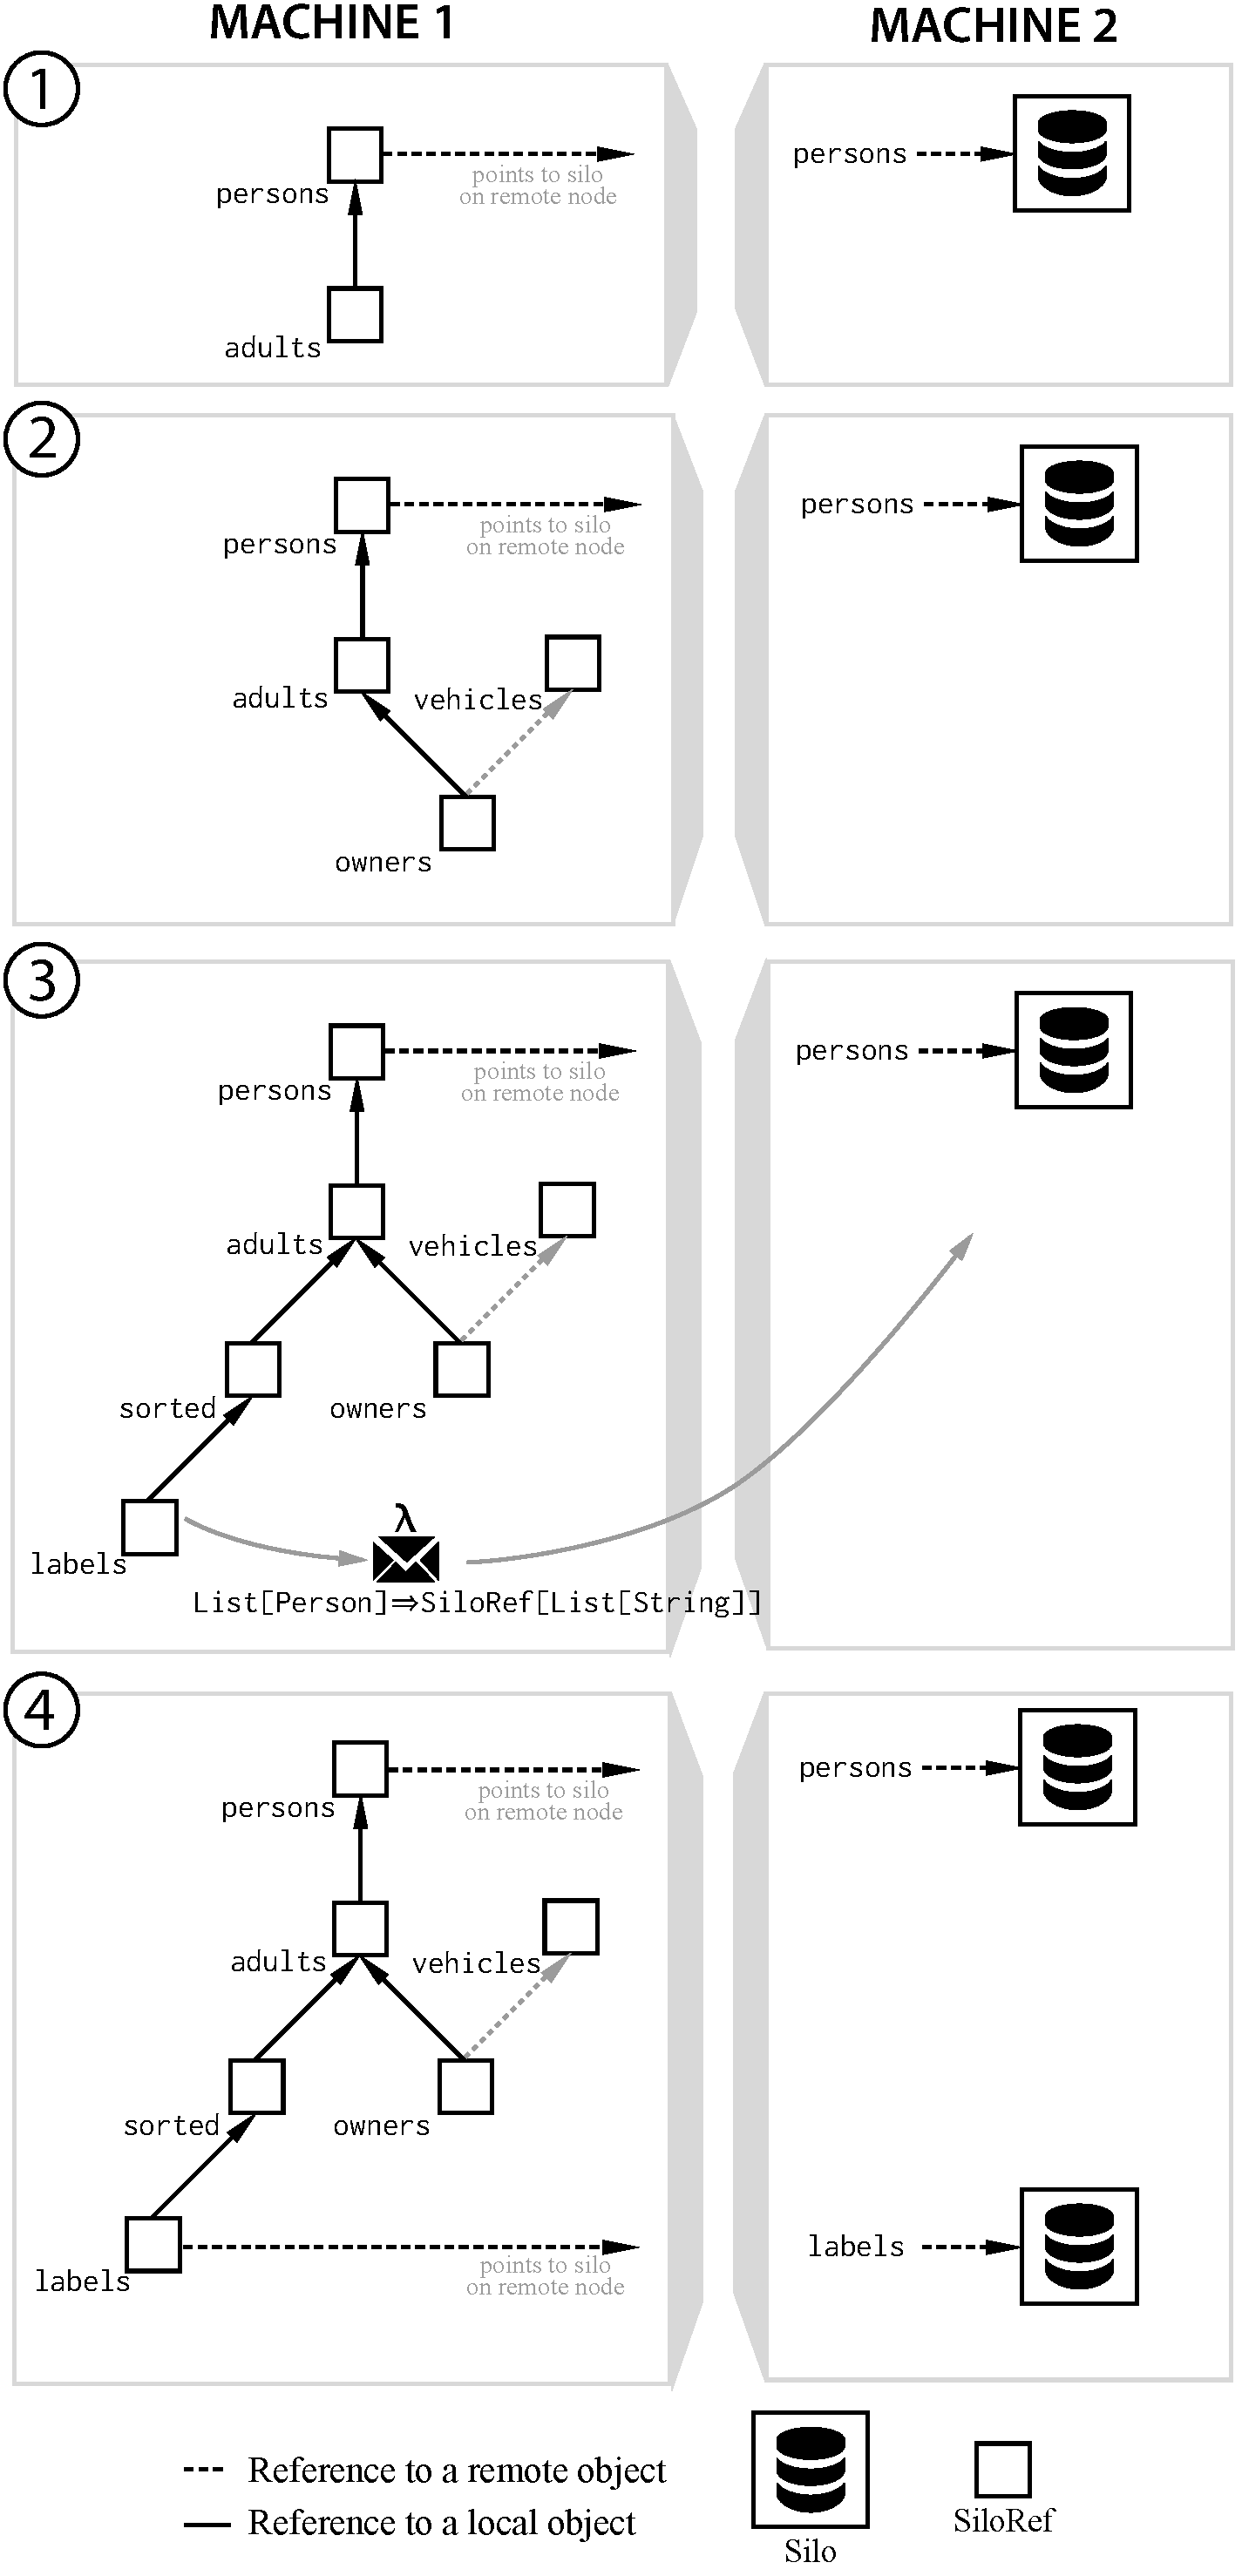
\includegraphics[scale=0.35]{pic/bigger-dag.pdf}
\caption{Matching persons and vehicle owners using the \texttt{apply} combinator.}\label{fig:apply-illustrated}
\end{figure}

\subsection{K-Means Clustering}\label{app:kmeans-illustrated}

Figure~\ref{fig:kmeans-illustrated} shows an illustrated version of
the listing of the k-means clustering example in
Section~\ref{sec:mbrace}.

\begin{figure}[ht!]
\centering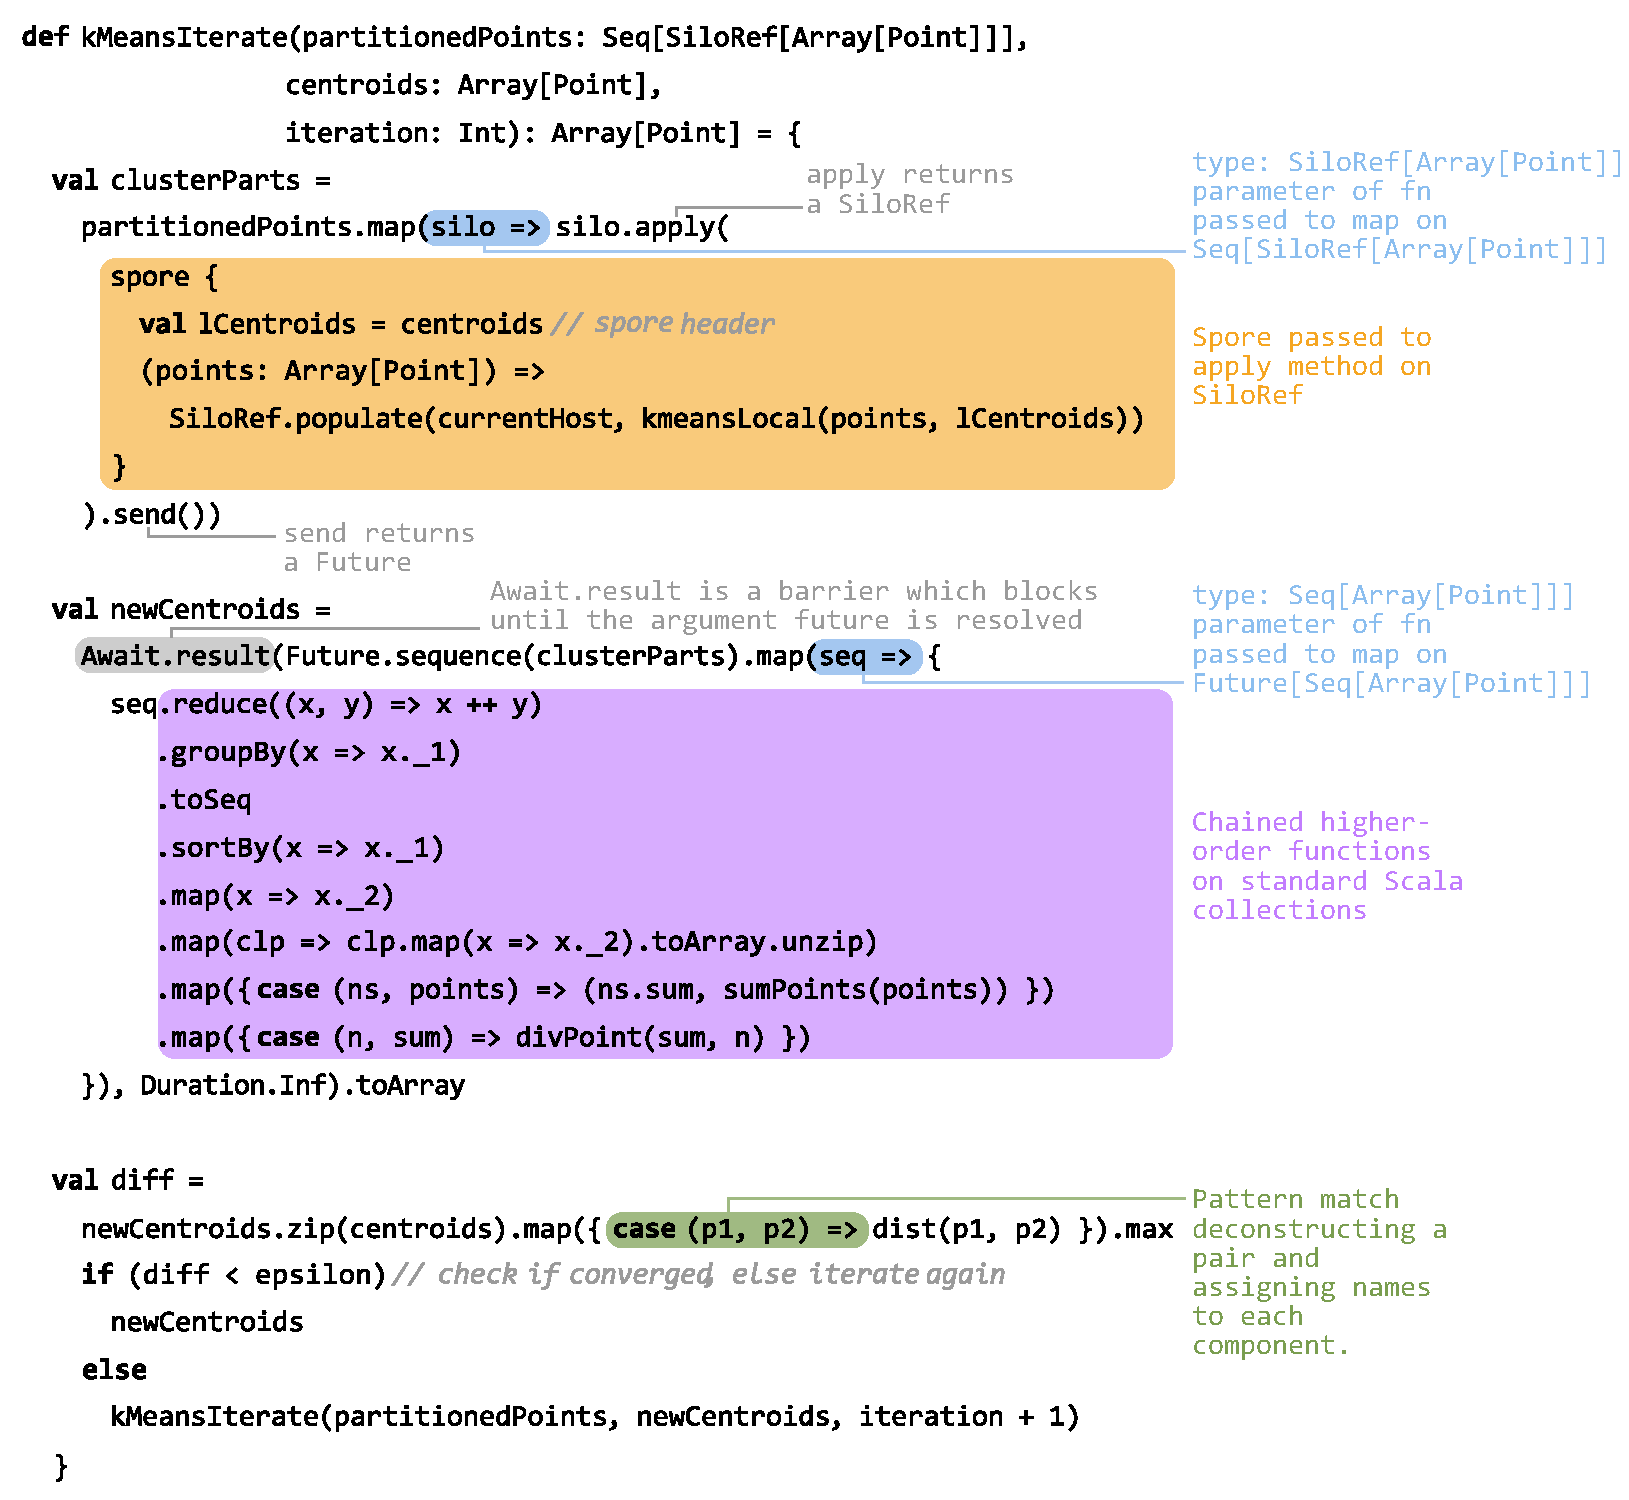
\includegraphics[scale=0.46]{k-means-annotated.pdf}
\caption{Excerpt of an implementation of k-means
  clustering.}\label{fig:kmeans-illustrated}
\end{figure}

\newpage
\section{Proofs}

\subsection{Proof of Theorem~\ref{lem:ser-values}}\label{app:ser-values}

\begin{thmun}
\emph{(Serializable Values)}
If $\Gamma ; \Sigma \vdash v : T$ and $serializable(T)$ then $\emptyset ; \Sigma \vdash v : T$.
\end{thmun}
\begin{proof}
By induction on the derivation of $\Gamma ; \Sigma \vdash v : T$ with a case analysis of the last applied rule.

\begin{itemize}
\item Cases \textsc{T-Int}, \textsc{T-Unit}, and \textsc{T-Host} are trivial.

\item Case \textsc{T-SiloRef}.
\begin{enumerate}
% 1.
\item By the assumptions
  \begin{enumerate}[label=(\alph*)]
  \item $\Gamma ; \Sigma \vdash v : T$
  \item $serializable(T)$
  \end{enumerate}
% 2.
\item By 1.a) and \textsc{T-SiloRef}
  \begin{enumerate}[label=(\alph*)]
  \item $v = {\Ref l h}$
  \item $T = \SR{T'}$
  \item $\Sigma(id(l)) = T'$
  \item $\Sigma \vdash {\Ref l h}$
  \end{enumerate}
% 3.
\item By 2.a-d), and \textsc{T-SiloRef}, $\emptyset ; \Sigma \vdash v : T$.
\end{enumerate}

\item Case \textsc{T-Spore} follows by \textsc{S-Spore} and the IH.
\end{itemize}
\end{proof}


\subsection{Proof of Theorem~\ref{th:subject-reduction}}\label{app:subject-reduction}

\begin{lem}
\emph{(Weakening)}\label{lem:weakening}
If $\Gamma ; \Sigma \vdash t : T$ and $x \notin dom(\Gamma)$, then
$\Gamma , x : T' ; \Sigma \vdash t : T$.
\end{lem}
\begin{proof}
By induction on the derivation of $\Gamma ; \Sigma \vdash t : T$.
\end{proof}

\begin{lem}
\emph{(Weakening of Store Typing)}\label{lem:weakening-store-typing}
\begin{enumerate}
\item If $\Gamma ; \Sigma \vdash t : T$ and $\iota \notin \mathit{dom}(\Sigma)$ then $\Gamma ; \Sigma' \vdash t : T$ where $\Sigma' = [\iota \mapsto T']\Sigma$.
\item If $\Sigma \vdash (t, \sigma)^h$ and $\iota \notin \mathit{dom}(\Sigma)$ then $\Sigma' \vdash (t, \sigma)^h$ where $\Sigma' = [\iota \mapsto T]\Sigma$.
\item If $\Sigma \vdash H$ and $\iota \notin \mathit{dom}(\Sigma)$ then $\Sigma' \vdash H$ where $\Sigma' = [\iota \mapsto T]\Sigma$.
\end{enumerate}
\end{lem}
\begin{proof}
Part 1: By induction on the derivation of $\Gamma ; \Sigma \vdash t : T$. Part 2: By induction on the derivation of $\Sigma \vdash (t, \sigma)^h$. Part 3: By induction on the derivation of $\Sigma \vdash H$.
\end{proof}

\begin{lem}\emph{(Process)}\label{lem:process}
If $\Sigma \vdash \sigma$, $\Sigma \vdash m$, and $process(h, m, \sigma) = (t, M, \sigma')$ then $\emptyset ; \Sigma' \vdash t : T$ for some $T$, $\Sigma' \vdash M$, and $\Sigma' \vdash \sigma'$ for some $\Sigma' \supseteq \Sigma$.
\end{lem}
\begin{proof}
\begin{itemize}
\item Case \textsc{Proc-Req}.
\begin{enumerate}
% 1.
\item By the assumptions
  \begin{enumerate}[label=(\alph*)]
  \item $\Sigma \vdash \sigma$
  \item $\Sigma \vdash m$
  \item $process(h, m, \sigma) = (t, M, \sigma')$
  \end{enumerate}
% 2.
\item By \textsc{Proc-Req}
  \begin{enumerate}[label=(\alph*)]
  \item $m = {\Req {h'} r \iota}$
  \item $r = {\Ref l h}$
  \item $\sigma(id(l)) = (v, P)$
  \item $M = \{ h' \leftarrow {\Res \iota v} \}$
  \item $\sigma' = {\consume {id(l)} P \sigma}$
  \item $t = \texttt{unit}$
  \end{enumerate}
% 3.
\item Define $\Sigma' := \Sigma$.
% 4.
\item By 2.e) and Def.~\ref{def:consume}, $dom(\sigma') \subseteq dom(\sigma)$.
% 5.
\item By 1.a), 3., 4., and \textsc{WF-Store1-3}, $\Sigma' \vdash \sigma'$.
% 6.
\item By 1.b), 2.a,b), and \textsc{WF-Req}
  \begin{enumerate}[label=(\alph*)]
  \item $\Sigma(id(l)) = \Sigma(\iota)$
  \item $\Sigma \vdash r$
  \end{enumerate}
% 7.
\item Define $T := \Sigma(id(l))$.
% 8.
\item By 1.a), 2.c), 7., and \textsc{WF-Store2}, $\emptyset ; \Sigma \vdash v : T$.
% 9.
\item By 6.a), 7., 8., and \textsc{WF-Res}, $\Sigma \vdash {\Res \iota v}$.
% 10.
\item By 2.d), 9., and \textsc{WF-Messages}, $\Sigma \vdash M$.
% 11.
\item By 2.f), \textsc{T-Unit}, and Lemma~\ref{lem:weakening-store-typing}, $\emptyset ; \Sigma \vdash t : T'$ for some $T'$.
% 12.
\item 3., 5., 10., and 11. close this case.
\end{enumerate}

\item Cases \textsc{Proc-ReqMat1}, \textsc{Proc-ReqMat2}, and \textsc{Proc-ReqParent} follow analogously.

\item Case \textsc{Proc-ReqApply}.
\begin{enumerate}
% 1.
\item By the assumptions
  \begin{enumerate}[label=(\alph*)]
  \item $\Sigma \vdash \sigma$
  \item $\Sigma \vdash m$
  \item $process(h, m, \sigma) = (t, M, \sigma')$
  \end{enumerate}
% 2.
\item By \textsc{Proc-ReqApply}
  \begin{enumerate}[label=(\alph*)]
  \item $m = {\Req {h'} r \iota}$
  \item $r = {\Ref l h}$
  \item $l = {\FMapped {\iota'} {l'} p}$
  \item $\sigma(id(l')) = (v, P)$
  \item $t = \texttt{respond}(h', \iota, \texttt{await}(\texttt{send}(p~v)))$
  \item $\sigma' = {\consume {id(l')} P \sigma}$
  \item $M = \emptyset$
  \end{enumerate}
% 3.
\item By 1.b), 2.a,b), and \textsc{WF-Req}
  \begin{enumerate}[label=(\alph*)]
  \item $\Sigma(id(l)) = \Sigma(\iota)$
  \item $\Sigma \vdash r$
  \end{enumerate}
% 4.
\item By 2.b,c), 3.b), \textsc{WF-Ref}, and \textsc{WF-Lin2}
  \begin{enumerate}[label=(\alph*)]
  \item $\Sigma(\iota') = T$
  \item $\Sigma(id(l')) = T'$
  \item $\exists \Gamma.~\Gamma ; \Sigma \vdash p : T' \Rightarrow \texttt{SiloRef}[T]~\{\ldots\}$
  \item $\Sigma \vdash l'$
  \end{enumerate}
% 5.
\item By 1.a), 2.d), 4.b), and \textsc{WF-Store2}, $\emptyset ; \Sigma \vdash v : T'$.
% 6.
\item By 4.c), \textsc{T-Spore}, Def.~$serializable$, and Lemma~\ref{lem:ser-values}, $\emptyset ; \Sigma \vdash p : T' \Rightarrow \texttt{SiloRef}[T]~\{\ldots\}$.
% 7.
\item By 5., 6., and \textsc{T-AppSpore}, $\emptyset, \Sigma \vdash p~v : \texttt{SiloRef}[T]$.
% 8.
\item By 7. and \textsc{T-Send}, $\emptyset, \Sigma \vdash \texttt{send}(p~v) : \texttt{Future}[T]$.
% 9.
\item By 8. and \textsc{T-Await}, $\emptyset, \Sigma \vdash \texttt{await}(\texttt{send}(p~v)) : T$.
% 10.
\item By 3.a), 4.a), and Def.~\ref{def:id}, $\Sigma(\iota) = T$ and thus by \textsc{T-Ident}, $\emptyset ; \Sigma \vdash \iota : \texttt{Future}[T]$.
% 11.
\item By 2.e), 9., 10., and \textsc{T-Respond}, $\emptyset, \Sigma \vdash t : \texttt{Unit}$.
% 12.
\item By 2.g) and \textsc{WF-Messages-Emp}, $\Sigma \vdash M$.
% 13.
\item By 2.f) and Def.~\ref{def:consume}, $dom(\sigma') \subseteq dom(\sigma)$.
% 14.
\item By 1.a), 13., and \textsc{WF-Store1-3}, $\Sigma \vdash \sigma'$.
% 15.
\item 11., 12., and 14. close this case.
\end{enumerate}

% TODO: expand for debugging
\item Cases \textsc{Proc-ReqPersist} and \textsc{Proc-Res} follow analogously.

\end{itemize}
\end{proof}


\begin{thmun}
\emph{(Subject Reduction)}

\begin{enumerate}

\item If $\Gamma ; \Sigma \vdash t : T$, $\Sigma \vdash \sigma$, and $t~|~\sigma \rightarrow^h t'~|~\sigma'$ then $\Gamma ; \Sigma' \vdash t' : T$ and $\Sigma' \vdash \sigma'$ for some $\Sigma' \supseteq \Sigma$.

\item If $\Sigma \vdash H~|~M$ and $H~|~M \twoheadrightarrow H'~|~M'$ then $\Sigma' \vdash H'~|~M'$ for some $\Sigma' \supseteq \Sigma$.

\end{enumerate}

\end{thmun}
\begin{proof}

Part 1: by induction on the derivation of $t~|~\sigma \rightarrow^h t'~|~\sigma'$ with case analysis of the last applied rule.

\begin{itemize}
\item Case \textsc{R-AppAbs}.
\begin{enumerate}
% 1.
\item By the assumptions
  \begin{enumerate}[label=(\alph*)]
  \item $\Gamma ; \Sigma \vdash t : T$
  \item $\Sigma \vdash \sigma$
  \item $t~|~\sigma \rightarrow^h t'~|~\sigma'$
  \end{enumerate}
% 2.
\item By \textsc{R-AppAbs}
  \begin{enumerate}[label=(\alph*)]
  \item $t = E[((x : T') \Rightarrow t'')~v']$
  \item $t' = E[[x \mapsto v']t'']$
  \item $\sigma' = \sigma$
  \end{enumerate}
% 3.
\item By 1.a) and 2.a), $\Gamma ; \Sigma \vdash ((x : T') \Rightarrow t'')~v' : T''$.
% 4.
\item By 3. and \textsc{T-App},
  \begin{enumerate}[label=(\alph*)]
  \item $\Gamma ; \Sigma \vdash ((x : T') \Rightarrow t'') : T' \Rightarrow T''$
  \item $\Gamma ; \Sigma \vdash v' : T'$
  \end{enumerate}
% 5.
\item By 4.a) and \textsc{T-Abs}, $\Gamma , x : T' ; \Sigma \vdash t'' : T''$.
% 6.
\item By 4.b), 5., and Lemma~\ref{th:subst}, $\Gamma ; \Sigma \vdash [x \mapsto v']t'' : T''$.
% 7.
\item By 1.a), 2.a-b), 3., and 6., $\Gamma ; \Sigma \vdash t' : T$.
% 8.
\item 2.c) and 7. close this case.
\end{enumerate}

\item Cases \textsc{R-IntOp}, \textsc{R-AppSpore}, and \textsc{R-Await} follow analogously.

\item Case \textsc{R-Apply}.
\begin{enumerate}
% 1.
\item By the assumptions
  \begin{enumerate}[label=(\alph*)]
  \item $\Gamma ; \Sigma \vdash t : T$
  \item $\Sigma \vdash \sigma$
  \item $t~|~\sigma \rightarrow^h t'~|~\sigma'$
  \end{enumerate}
% 2.
\item By \textsc{R-Apply}
  \begin{enumerate}[label=(\alph*)]
  \item $t  = E[\texttt{apply}(r, p)]$
  \item $r  = {\Ref l {h'}}$
  \item $t' = E[r']$
  \item $r' = {\Ref {l'} {h'}}$
  \item $l' = {\FMapped {(h, i)} l p}$ where $i~\text{fresh}$
  \item $\sigma' = \sigma$
  \end{enumerate}
% 3.
\item By 1.a) and 2.a), $\Gamma ; \Sigma \vdash \texttt{apply}(r, p) : \hat{T}$.
% 4.
\item By 3. and \textsc{T-Apply},
  \begin{enumerate}[label=(\alph*)]
  \item $\hat{T} = \texttt{SiloRef}[T']$
  \item $\Gamma ; \Sigma \vdash r : \texttt{SiloRef}[T'']$
  \item $\Gamma ; \Sigma \vdash p : T'' \Rightarrow \texttt{SiloRef}[T']~\{~\texttt{type}~\mathcal{C} = \seq{T}~\}$
  \end{enumerate}
% 5.
\item By 2.b), 4.b), \textsc{T-SiloRef}, and \textsc{WF-Ref}
  \begin{enumerate}[label=(\alph*)]
  \item $\Sigma(id(l)) = T''$
  \item $\Sigma \vdash r$
  \item $\Sigma \vdash l$
  \item $h' \in \mathcal{H}$
  \end{enumerate}
% 6.
\item Define $\Sigma' := [(h, i) \mapsto T']\Sigma$.
% 7.
\item By 2.d-e), 4.c), 5.a-d), 6., \textsc{WF-Lin2}, and \textsc{WF-Ref}, $\Sigma' \vdash r'$.
% 8.
\item By 2.d-e), 6., 7., and \textsc{T-SiloRef}, $\Gamma ; \Sigma' \vdash r' : \texttt{SiloRef}[T']$.
% 9.
\item By 2.e), 3., 4.a), 6., and part 1 of Lemma~\ref{lem:weakening-store-typing}, $\Gamma ; \Sigma' \vdash \texttt{apply}(r, p) : \texttt{SiloRef}[T']$.
% 10.
\item By 1.a), 2.e), 6., and part 1 of Lemma~\ref{lem:weakening-store-typing}, $\Gamma ; \Sigma' \vdash t : T$.
% 11.
\item By 2.a,c), 8., 9., and 10., $\Gamma ; \Sigma' \vdash t' : T$.
% 12.
\item By 1.b) and 2.f), $\Sigma \vdash \sigma'$.
% 13.
\item By 6., $\Sigma' \supseteq \Sigma$.
% 14.
\item By 12., 13., and \textsc{WF-Store3}, $\Sigma' \vdash \sigma'$.
% 15.
\item 11., 13., and 14. close this case.

\end{enumerate}

\item Cases \textsc{R-Persist} and \textsc{R-Unpersist} follow analogously.
\end{itemize}

%
Part 2: by induction on the derivation of $H~|~M \twoheadrightarrow H'~|~M'$ with case analysis of the last applied rule.

\begin{itemize}
\item Case \textsc{R-Local}.
\begin{enumerate}
% 1.
\item By the assumptions
  \begin{enumerate}[label=(\alph*)]
  \item $\Sigma \vdash H~|~M$
  \item $H~|~M \twoheadrightarrow H'~|~M'$
  \end{enumerate}
% 2.
\item By \textsc{R-Local}
  \begin{enumerate}[label=(\alph*)]
  \item $H = \{ (t, \sigma)^h \} \cup H''$
  \item $H' = \{ (t', \sigma')^h \} \cup H''$
  \item $t~|~\sigma \rightarrow^h t'~|~\sigma'$
  \item $M' = M$
  \end{enumerate}
% 3.
\item By 1.a) and \textsc{WF-Config}, $\Sigma \vdash H$.
% 4.
\item By 2.a), 3., and \textsc{WF-Host2}
  \begin{enumerate}[label=(\alph*)]
  \item $\Sigma \vdash (t, \sigma)^h$
  \item $\Sigma \vdash H''$
  \end{enumerate}
% 5.
\item By 4.a) and \textsc{WF-HostConfig}
  \begin{enumerate}[label=(\alph*)]
  \item $\Sigma \vdash \sigma$
  \item $\Gamma ; \Sigma \vdash t : T$ for some $\Gamma$
  \end{enumerate}
% 6.
\item By 2.c), 5.a,b), and part 1
  \begin{enumerate}[label=(\alph*)]
  \item $\Gamma ; \Sigma' \vdash t' : T$
  \item $\Sigma' \vdash \sigma'$ for some $\Sigma' \supseteq \Sigma$
  \end{enumerate}
% 7.
\item By 6.a,b) and \textsc{WF-HostConfig}, $\Sigma' \vdash (t', \sigma')^h$.
% 8.
\item By 4.b), 6.b), and part 3 of Lemma~\ref{lem:weakening-store-typing}, $\Sigma' \vdash H''$.
% 9.
\item By 2.b), 7., 8., and \textsc{WF-Host2}, $\Sigma' \vdash H'$.
% 10.
\item By 1.a), 2.d), 9., \textsc{WF-Config}, and \textsc{WF-Messages}, $\Sigma' \vdash H'~|~M'$.
\end{enumerate}

\item Case \textsc{R-Send}.
\begin{enumerate}
% 1.
\item By the assumptions
  \begin{enumerate}[label=(\alph*)]
  \item $\Sigma \vdash H~|~M$
  \item $H~|~M \twoheadrightarrow H'~|~M'$
  \end{enumerate}
% 2.
\item By \textsc{R-Send}
  \begin{enumerate}[label=(\alph*)]
  \item $H  = \{ (E[\texttt{send}(r)], \sigma)^h \} \cup H''$
  \item $H' = \{ (E[id(l)], \sigma)^h \} \cup H''$
  \item $r  = {\Ref l {h'}}$
  \item $m  = {\Req h r {id(l)}}$
  \item $M' = M \uplus \{ h' \leftarrow m \}$
  \end{enumerate}
% 3.
\item By 1.a) and \textsc{WF-Config}
  \begin{enumerate}[label=(\alph*)]
  \item $\Sigma \vdash H$
  \item $\Sigma \vdash M$
  \end{enumerate}
% 4.
\item By 2.a), 3.a), and \textsc{WF-Host2}
  \begin{enumerate}[label=(\alph*)]
  \item $\Sigma \vdash (E[\texttt{send}(r)], \sigma)^h$
  \item $\Sigma \vdash H''$
  \end{enumerate}
% 5.
\item By 4.a) and \textsc{WF-HostConfig}
  \begin{enumerate}[label=(\alph*)]
  \item $\Sigma \vdash \sigma$
  \item $\Gamma ; \Sigma \vdash E[\texttt{send}(r)] : T$ for some $\Gamma$
  \end{enumerate}
% 6.
\item By 5.b), $\Gamma ; \Sigma \vdash \texttt{send}(r) : \hat{T}$.
% 7.
\item By 6. and \textsc{T-Send}
  \begin{enumerate}[label=(\alph*)]
  \item $\hat{T} = \texttt{Future}[T'']$
  \item $\Gamma ; \Sigma \vdash r : \texttt{SiloRef}[T'']$
  \end{enumerate}
% 8.
\item By 2.c), 7.b), and \textsc{T-SiloRef}
  \begin{enumerate}[label=(\alph*)]
  \item $\Sigma(id(l)) = T''$
  \item $\Sigma \vdash r$
  \end{enumerate}
% 9.
\item By 8.a) and \textsc{T-Ident}, $\Gamma ; \Sigma \vdash id(l) : \texttt{Future}[T'']$.
% 10.
\item By 5.b), 6., 7.a), and 9., $\Gamma ; \Sigma \vdash E[id(l)] : T$.
% 11.
\item By 5.a), 10., and \textsc{WF-HostConfig}, $\Sigma \vdash (E[id(l)], \sigma)^h$.
% 12.
\item By 4.b), 11., and \textsc{WF-Host2}, $\Sigma \vdash H'$.
% 13.
\item By 2.c,d), 8.b), and \textsc{WF-Req}, $\Sigma \vdash m$.
% 14.
\item By 2.c,e), 3.b), 8.b), 13., \textsc{WF-Ref}, and \textsc{WF-Messages}, $\Sigma \vdash M'$.
% 15.
\item By 12., 14., and \textsc{WF-Config}, $\Sigma \vdash H'~|~M'$.
\end{enumerate}

\item Cases \textsc{R-Populate} and \textsc{R-Respond} follow analogously.

\item Case \textsc{R-Process}.
\begin{enumerate}
% 1.
\item By the assumptions
  \begin{enumerate}[label=(\alph*)]
  \item $\Sigma \vdash H~|~M$
  \item $H~|~M \twoheadrightarrow H'~|~M'$
  \end{enumerate}
% 2.
\item By \textsc{R-Process}
  \begin{enumerate}[label=(\alph*)]
  \item $H  = \{ (E[\texttt{await}(\iota)], \sigma)^h \} \cup H''$
  \item $H' = \{ (E[t~;~\texttt{await}(\iota)], \sigma')^h \} \cup H''$
  \item $M' = \hat{M} \uplus M''$
  \item $process(h, m, \sigma) = (t, M'', \sigma')$
  \item $M = \hat{M} \uplus \{ h \leftarrow m \}$
  \end{enumerate}
% 3.
\item By 1.a) and \textsc{WF-Config}
  \begin{enumerate}[label=(\alph*)]
  \item $\Sigma \vdash H$
  \item $\Sigma \vdash M$
  \end{enumerate}
% 4.
\item By 2.a), 3.a), and \textsc{WF-Host2}
  \begin{enumerate}[label=(\alph*)]
  \item $\Sigma \vdash (E[\texttt{await}(\iota)], \sigma)^h$
  \item $\Sigma \vdash H''$
  \end{enumerate}
% 5.
\item By 4.a) and \textsc{WF-HostConfig}
  \begin{enumerate}[label=(\alph*)]
  \item $\Sigma \vdash \sigma$
  \item $\Gamma ; \Sigma \vdash E[\texttt{await}(\iota)] : T$ for some $\Gamma$
  \end{enumerate}
% 6.
\item By 2.e), 3.b), and \textsc{WF-Messages}, $\Sigma \vdash m$.
% 7.
\item By 2.d), 5.a), 6., and Lemma~\ref{lem:process}~(Process), $\exists \Sigma'$ such that
  \begin{enumerate}[label=(\alph*)]
  \item $\emptyset ; \Sigma' \vdash t : T'$
  \item $\Sigma' \vdash M''$
  \item $\Sigma' \vdash \sigma'$
  \item $\Sigma' \supseteq \Sigma$
  \end{enumerate}
% 8.
\item By 5.b), 7.d), and part 1 of Lemma~\ref{lem:weakening-store-typing}, $\Gamma ; \Sigma' \vdash E[\texttt{await}(\iota)] : T$.
% 9. XXX
\item By 7.a) and 8., $\Gamma ; \Sigma' \vdash E[t~;~\texttt{await}(\iota)] : T$.
% 10.
\item By 7.c), 9., and \textsc{WF-HostConfig}, $\Sigma' \vdash (E[t~;~\texttt{await}(\iota)], \sigma')^h$.
% 11.
\item By 4.b), 7.d), and part 3 of Lemma~\ref{lem:weakening-store-typing}, $\Sigma' \vdash H''$.
% 12.
\item By 2.b), 10., 11., and \textsc{WF-Host2}, $\Sigma' \vdash H'$.
% 13.
\item By 3.b), 7.d), \textsc{WF-Res}, \textsc{WF-Req}, \textsc{WF-Ref}, and \textsc{WF-Messages}, $\Sigma' \vdash M$.
% 14.
\item By 2.c), 7.b), 13., and \textsc{WF-Messages}, $\Sigma' \vdash M'$.
% 15.
\item By 12., 14., and \textsc{WF-Config}, $\Sigma' \vdash H'~|~M'$.
\end{enumerate}

\item Case \textsc{R-Process-Val} follows analogously.

\end{itemize}

\end{proof}

\subsection{Proof of Theorem~\ref{thm:finite-mat}}\label{app:finite-mat}

\begin{lem}[Responsive Population]\label{lem:resp-population}
  Let $\Sigma \vdash H~|~M~|~R$ and $H = \{ (E[t], \sigma)^h \} \uplus
  \hat{H}$.

  Then $\forall h' \in \mathit{hosts}(H)$: $\{ (E[\texttt{send}(r)],
  \sigma)^h \} \uplus \hat{H}~|~M \uplus \{ h' \leftarrow m \}
  \twoheadrightarrow^* H'~|~M' \uplus \{ h \leftarrow m \}$ after a
  finite number of reduction steps where $r = {\Ref l {h'}}$, $l =
  {\Mat \iota}$ for some $\iota$, and $m = {\Res \iota v}$.
\end{lem}
\begin{proof}[Proof Sketch]
  By \textsc{R-Send}, $\{ (E[\texttt{send}(r)], \sigma)^h \} \uplus
  \hat{H}~|~M \uplus \{ h' \leftarrow m \} \twoheadrightarrow \{
  (E[\iota], \sigma)^h \} \uplus \hat{H}~|~M \uplus \{ h' \leftarrow m
  \} \uplus \{ h' \leftarrow m' \}$ where $m' = {\Req h r \iota}$.
  By Def.~\ref{def:fair-scheduling} message $m$ is processed by $h'$
  after a finite number of reduction steps. As a result, the store of
  $h'$ is updated with the mapping $\iota \mapsto v$. After another
  finite number of reduction steps, $h'$ processes message $m'$. By
  \textsc{R-Process}, \textsc{R-Process-Val}, and
  \textsc{Proc-ReqMat1}, the resulting multiset of messages includes
  $\{h \leftarrow {\Res \iota v} \}$ as required.
\end{proof}

\begin{lem}[Responsive Apply]\label{lem:resp-apply}
\end{lem}
\begin{proof}
\begin{enumerate}
  % 1.
\item By \textsc{R-Local} and \textsc{R-Apply}
  \begin{enumerate}[label=(\alph*)]
  \item $E[\texttt{apply}(r, p)]~|~\sigma \rightarrow^h E[r']~|~\sigma~|~\{ r' \}$
  \item $r' = {\Ref {l'} {h'}}$
  \item $r = {\Ref l {h'}}$
  \item $l' = {\FMapped {(h, i)} l p}$ where $i$ fresh
  \item $H' = \{ (E[r'], \sigma)^h \} \uplus \hat{H}$
  \item $M' = M$
  \item $R' = R \uplus \{ r' \}$
  \end{enumerate}
  % 2.
\item By Lemma~\ref{lem:resp}, $\mathit{Responsive}(H', M', R)$.
  % 3.
\item Consider $H'~|~M' \uplus \{h' \leftarrow m\}~|~R'$ where $m =
  {\Req {h''} {r'} \iota}$.
  % 4.
\item By Def.~\ref{def:fair-scheduling} $H'~|~M' \uplus \{h'
  \leftarrow m\}~|~R' \twoheadrightarrow^* H_p~|~M_p~|~R_p$ such that
  $(E_p[\texttt{await}(\iota_p)], \sigma_p)^{h'} \in H_p \lor
  (E_p[v_p], \sigma_p)^{h'} \in H_p$ and $\{h' \leftarrow m\} \in
  M_p$.
  % 5.
\item There are two cases. {\em Case 1:} $id(l) \notin
  \mathit{dom}(\sigma')$. In this case $H_p~|~M_p~|~R_p$ can be
  reduced according to \textsc{R-Process} (or \textsc{R-Process-Val})
  and \textsc{Proc-ReqParent}. As a result, $h'$ reduces
  $\texttt{send}({\Ref l {h'}})$. By \textsc{R-Send}, ${\Ref l {h'}}
  \in R$, and Lemma~\ref{lem:resp}, $H_p~|~M_p~|~R_p
  \twoheadrightarrow^* H_r~|~M_r \uplus \{h' \leftarrow {\Res {id(l)}
    v} \}~|~R_r$ after a finite number of reduction steps. By
  Def.~\ref{def:fair-scheduling} and \textsc{Proc-Res}, $H_r~|~M_r
  \uplus \{h' \leftarrow {\Res {id(l)} v} \}~|~R_r
  \twoheadrightarrow^* H''~|~M''~|~R''$ after a finite number of
  reduction steps, such that
  \begin{enumerate}[label=(\alph*)]
  \item $H'' = \{ (E'[t'], \sigma')^{h'} \} \cup H_3$ where $t' = v'$
    or $t' = \texttt{await}(\iota')$
  \item $M'' = \{h' \leftarrow m\} \uplus M_3$
  \item $\sigma'(id(l)) = v$
  \item $\Sigma'' \vdash H''~|~M''~|~R''$
  \end{enumerate}
  {\em Case 2:} $\sigma'(id(l)) = v$. In this case $H'' = H_p$, $M'' =
  M_p$, and $R'' = R_p$.
  % 6.
\item By 5.a-c), \textsc{R-Process}, \textsc{R-Process-Val}, and
  \textsc{Proc-ReqApply}
  \begin{enumerate}[label=(\alph*)]
  \item $\mathit{process}(h', m, \sigma') = (t'', \emptyset, \sigma')$
  \item $t'' = \texttt{respond}(h'', \iota, \texttt{await}(\texttt{send}(p~v)))$
  \item $H''~|~M''~|~R'' \twoheadrightarrow H_3~|~M_3~|~R''$
  \item $H_3 = \{ (E'[t''~\texttt{;}~t'], \sigma')^{h'} \} \cup H_4$
  \end{enumerate}
  % 7.
\item By 5.d), 6.c), and Theorem~\ref{th:subject-reduction} (Subject
  Reduction), $\Sigma_3 \vdash \{ (E'[t''~\texttt{;}~t'],
  \sigma')^{h'} \} \cup H_4~|~M_3~|~R''$ for some $\Sigma_3 \supseteq
  \Sigma''$.
  % 8.
\item By 7., \textsc{WF-Config}, \textsc{WF-Host2}, and \textsc{WF-HostConfig}
  \begin{enumerate}[label=(\alph*)]
  \item $\Sigma_3 \vdash \sigma'$
  \item $\Gamma_3 ; \Sigma_3 \vdash E'[t''~\texttt{;}~t'] : T_3$ for
    some $\Gamma_3$, $T_3$
  \end{enumerate}
  % 9.
\item By 6.b), 8.b), and the type rules
  \begin{enumerate}[label=(\alph*)]
  \item $\Gamma_4 ; \Sigma_3 \vdash p : T' \Rightarrow \texttt{SiloRef}[T]~\{~\texttt{type}~\mathcal{C} = \seq{T}~\}$ for some $\Gamma_4$
  \item $p = \texttt{spore}~\{~\seq{x : T = v}~; (x: T') \Rightarrow t~\}$
  \end{enumerate}
  % 10.
\item By 9.a,b), and \textsc{T-Spore}
  \begin{enumerate}[label=(\alph*)]
  \item $\seq{x : T}, x : T' ; \emptyset \vdash t : \texttt{SiloRef}[T]$
  \item $\forall S \in \seq{T}, \texttt{SiloRef}[T].~\mathit{serializable}(S)$
  \end{enumerate}
  % 11.
  \item By the type rules, derivation 10.a) does not contain
    applications of \textsc{T-SiloRef} or \textsc{T-Ident}. By 10.b)
    spore $p$ does not capture futures. Thus, any occurrence of
    $\texttt{await}(\hat{\iota})$ within $p~v$ is preceded by a
    reduction of a corresponding $\texttt{send}$ resulting in future
    $\hat{\iota}$. By Lemma~\ref{lem:resp} (Responsiveness),
    $\mathit{Responsive}(H_3, M_3, R)$. There are two cases.

    {\em Case 1:} $d = 0$. Then $p$ does not contain a nested
    \texttt{apply} invocation. Therefore, by
    Lemma~\ref{lem:resp-population}, $p~v$ reduces to a value $r''$
    after a finite number of reduction steps. Since either $r'' \in R$
    or $r''$ is newly populated, $\texttt{send}(r'')$ results in a
    response $h' \leftarrow {\Res {id(r'')} {v''}}$ after a finite
    number of reduction steps. This enables $h'$ to reduce
    $\texttt{respond}(h'', \iota, v'')$ which concludes this case.

    {\em Case 2:} $d > 0$. The depth of nested \texttt{apply}s of
    term $p~v$ is less than the depth of the term $\texttt{apply}(r,
    p)$.  Therefore, by the induction hypothesis, reductions of nested
    \texttt{apply} invocations within $p~v$ result in responsive
    configurations. By Lemma~\ref{lem:resp-population}, $p~v$ reduces
    to a value $r''$ after a finite number of reduction steps. Since
    either $r'' \in R$, or $r''$ is newly populated, or $r''$ is the
    result of a nested \texttt{apply} invocation,
    $\texttt{send}(r'')$ results in a response $h' \leftarrow {\Res
      {id(r'')} {v''}}$ after a finite number of reduction steps. This
    enables $h'$ to reduce $\texttt{respond}(h'', \iota, v'')$ which
    concludes this case.
\end{enumerate}
\end{proof}

\begin{thmun}
\emph{(Finite Materialization)}
  Let $\Sigma \vdash H~|~M~|~R$ such that $\mathit{Responsive}(H, M,
  R)$.

  If $H~|~M~|~R \twoheadrightarrow H'~|~M'~|~R'$ then
  $\mathit{Responsive}(H', M', R')$.
\end{thmun}
\begin{proof}
  Corollary of Lemma~\ref{lem:resp}, Lemma~\ref{lem:resp-population},
  and Lemma~\ref{lem:resp-apply}.
\end{proof}
